The existence of this data system is paramount to several automation and system
health monitoring tasks in our lab. Below a few examples are described of the
use of the data system for these purposes. The examples given are how to create
a system health development graph from the continuously logged pressure data,
how we use the continuously logged data to monitor the health and status of
long duration experiments from home and finally how it can be used to create
alarms if some of the system parameters fall outside specified security ranges.

\subsection{Monitoring system health}
\label{sec:morning_pressure}
As mentioned in section \ref{sec:data_extraction} the flexibility of SQL
provides the possibility to do advanced data selection and very efficient
elementary data treatment directly in the database by means of the SQL query.
The can be used as in the example below, where the pressure in a vacuum
chamber at 1\,A.M. in the morning (where all the system parameters have settled
down) for the last month is extracted for plotting; 

\begin{verbatim} 
SELECT DATE(time), AVG(pressure) FROM pressure_microreactor WHERE hour(time) = 1 AND
minute(time) BETWEEN 00 AND 20 AND time BETWEEN {from} AND {to} GROUP BY
date(time) ORDER BY time DESC LIMIT 30; \end{verbatim} 

where \{from\} and \{to\} should be replaced with the relevant date interval.

The output from a statement such as the one above is illustrated in
Figure~\ref{fig:morning_pressure}.
\begin{figure}
 \begin{center}
 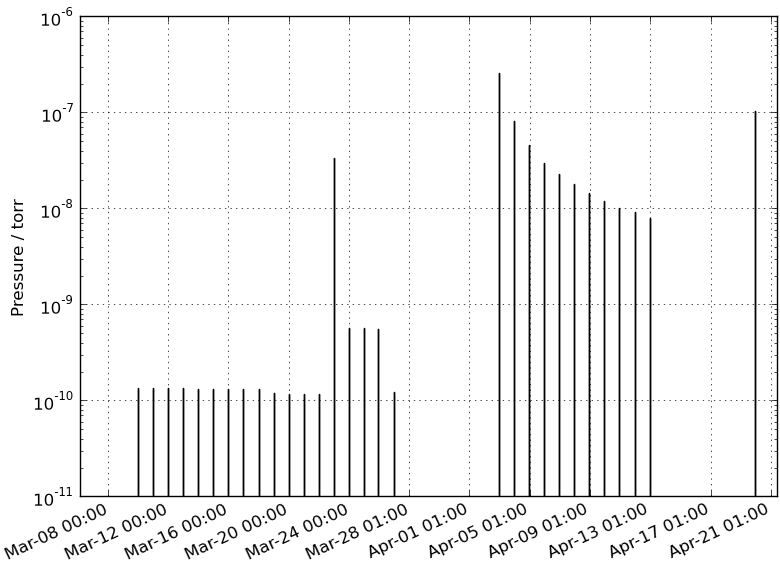
\includegraphics[width=10cm]{morning_pressure.png}
 \caption{ The morning pressure in a vacuum chamber at the department. The
   pressure gauge is unable to read high pressures, and thus no data is
   available from periods where the chamber is vented for maintenance.
   \label{fig:morning_pressure}
 } 
 \end{center} 
\end{figure} 
Plots like these can be a useful tool to monitor the general health of the
chamber, i.e. if leaks have developed, a valve is failing, a roughing pump is
malfunctioning etc. It should be mentioned that this is a function that have
been sought after for quite some time as ultra high vacuum is required for
surface science studies. Previously, this has simply not been possible before
the automated logging and selective plotting, as it would have required a
person to log the data in the middle of the night and to manually periodically
make new plots of the latest time period.

\subsection{Status of experiments with long durations} 
Within surface science it is not unusual to have experiments or a preparation
procedures before an experiment running for extended periods of time i.e.
overnight, or over several days. Obviously, for such procedures running when
no-one is present to monitor it, the programs that execute the procedure are
themselves responsible for the safety of the system/equipment and for shutting
it down if something unintentional happens. But with continuous logging, it is
now a simple task to add surveillance to these procedures that alerts the user
if the procedure has been stopped. When this happens, it is then possible for
the operator to access if it is safe to start the experiment again, even from
home. This can help to prevent a loss of experimentation time if the experiment
stopped e.g.\ during unsupervised experimentation time intervals like a
weekend.

One example where this is used is for the cleaning of metal single crystal
samples before experimentation. The cleaning of the surface is achieved by
running a number (5-20) of cleaning cycles. Each of these cycles can take up to
several hours. Before this task was automatized, it typically required simple
manual intervention 2-4 times during a 30 to 120 minute cycle. Obviously, this
was a suboptimal solution, since a lot of time was spent, with only small time
intervals to work on other things, before the next manual intervention. After
the total automation of the task and the implementation of the surveillance
features mentioned above this procedure can now run e.g.\ for 10-16 hours over
night and produce a sample ready for experimentation at the beginning of the
workday.

Another use of the monitoring of extended procedures are in the
experiments on microreactor setups~\cite{Henriksen2009}. For these devices,
it is very common to have quite long experimentation times. They can be used to
allow for sufficient system settle time when parameters have been changed, to
study long time stability effects on the samples or to thoroughly search the
parameter space for the experiment. Obviously, for all these purposes the more
experimentation time the better and being able to un-problematically and safely
utilize nights and weekends is a noticeable improvement.

\subsection{Cooling water alarms}\label{sec:cooling_water_alarms}

Several important pieces of equipment in our lab require cooling. If the
cooling disappears it can result in the break down of this equipment, which can
be quite expensive both in repair costs and lost equipment up-time. Using the
continuously logged data critical system parameters can be monitored and used
to trigger alarms when these fall out of specified ranges. To use this feature
to implement surveillance of the cooling temperature measurements on all the
equipment with critical cooling requirements have been mounted and all of these
temperatures logged via the data system. This approach has the desirable side
effect that system health can be monitored (to the extent it is given by the
temperature) of each piece of equipment individually to evaluate if the
equipment is getting old or requires maintenance. To implement the alarms a
program has been written that retrieves the latest temperatures from the
database, compares them with values from a previous time interval and sends out
an alarm via email if they increased out of range. Appropriately coupled with
email alarms, e.g.\ on smartphones, this feature provides the real-time user
notification of critical cooling loss.
